%%!TEX TS-program = xelatexmk
\documentclass[]{tufte-handout}

\usepackage{amsmath}
\usepackage{booktabs} % for tables
\usepackage{siunitx}
\usepackage{graphicx}
\usepackage{subfigure}
\usepackage{caption}
\usepackage{liecolon}
% Style for linguistic terms
\newcommand{\jgn}[1]{\textbf{\textsc{#1}}} 
%\newcommand{\jgn}[1]{\textsc{#1}} 
\usepackage{nicefrac}

\bibliographystyle{plain}


\title{FBPIC Benchmark test Against $m=0$ Hollow Channel Wake Fields}

\begin{document}
\maketitle

\section{Problem Statement}

\texttt{FBPIC}~\cite{lehe_etal:15} is an $r-z$ cylindrical electromagnetic particle-in-cell code with azimuthal modal decomposition designed for modeling laser plasma accelerators. The code is capable of arbitrary modal decompositions, i.e. $m=0, m=1, ...$ which makes it ideal for studying wake fields of order $m$ in a plasma accelerator, if it can accurately capture the wake fields. We are using the hollow plasma channel accelerator configuration as a benchmark, since the eigenmodes are known analytically\cite{schroeder_whittum_wurtele:1999}.


\begin{margintable}
\begin{tabular}{c c}
\hline
parameter & value [units] \\
\hline
channel\\
\hline
radius $b$ & \SI{20.}{\micro \meter} \\
density $n_e$ & \SI{1.e18}{\per \cubic \cm} \\
$k_p$ & \SI{188178.9}{\per \meter}\\
\hline
bunch \\
\hline
$\sigma_r$ & \SI{4.5}{\micro \meter} \\
$\sigma_z$ & \SI{9,}{\micro \meter} \\
$N_b$ & \num{1.e8} \\
\hline
\end{tabular}
\caption{\label{hcspecs}Hollow channel simulation parameters}
\end{margintable}

Our benchmark uses the parameters for the plasma and drive bunch in table~\ref{hcspecs}. These parameters sit in a regime where the drive bunch space charge does not strongly distort the hollow plasma channel. Reducing the density too much, or increasing the bunch charge too much, will break this comparison to the theory developed below.


\section{Hollow Plasma Channel Wake Functions}

The hollow plasma channel is a configuration for high gradient lepton accelerators. In the hollow channel, an empty annulus of plasma surrounds a drive bunch, akin to beam driven dielectric wakefield accelerators.

Once the hollow channel is formed, an analytic theory that treats the channel as a plasma with a hard edge can be applied. That theory predicts that the wake functions will be given by
\begin{subequations}
\begin{equation}
W_\parallel = - Q_{beam} \sum_m \frac{2 \kappa_m}{b^{2m}} \cos \left [\Omega_m k_p \zeta  \right ] a^m r^m \cos m \theta ~ \mathbf{e}_z
\end{equation}
\begin{equation}
W_\perp = - Q_{beam} \sum_m \frac{2 m \kappa_m}{b^{2m} \Omega_m k_p} \sin \left [\Omega_m k_p \zeta  \right ] r^{m-1} a^m \left [ \mathbf{e}_r \cos m \theta - \mathbf{e}_\theta \sin m \theta \right ]
\end{equation}
\end{subequations}
where $b$ is the channel radius, $\zeta$ is a longitudinal coordinate, $k_p = \omega_p/c$ is the channel plasma wavenumber, $Q_D$ is the drive bunch charge, and $\kappa_m$ and $\Omega_m$ are given by
\begin{subequations}
\begin{equation}
\kappa_m = k_p^2 \left [ \frac{K_m(k_p b)}{k_p b K_{m+1}(k_p b)} \right ]\left [1 + \frac{k_p b K_m(k_p b)}{2(m+1) K_{m+1}(k_p b)} \right ]^{-1}
\end{equation}
\begin{equation}
\Omega_m = \left [ \frac{(1 + \delta_{m,0}) (m+1) K_{m+1}(k_p b)}{2 (m+1) K_{m+1}(k_p b) + k_p b K_m(k_p b)} \right ]^{\nicefrac{1}{2}}
\end{equation}
\end{subequations}
where here $K_m$ is the $m^{th}$ modified Bessel function of the second kind.

For a gaussian beam with charge distribution
\begin{equation}
\rho(r, \zeta = z - c t) = \frac{Q_{beam}}{2 \pi \sigma_z \sigma_r^2} \exp \left [ - \frac{\zeta^2}{2 \sigma_z^2} \right ] \exp \left [ - \frac{r^2}{2 \sigma_r^2} \right ]
\end{equation}
the $m \neq 0$ wake fields all vanish due to azimuthal symmetry, and the $m=0$ longitudinal wake is given by
\begin{equation}
W_\parallel^{(0)} = - Q_{beam} \kappa_0 e^{-\frac{(\Omega_0 k_p \sigma_z)^2}{2}} \textrm{Re} \left (e^{- i \Omega_0 k_p \zeta} \textrm{Erfc} \left ( \frac{\zeta - i \Omega_0 k_p \sigma_z^2}{\sqrt{2} \sigma_z}\right ) \right )
\end{equation}

\section{FBPIC Simulations vs. Hollow Channel Theory}

Simulations using FBPIC show that FBPIC is able to get good agreement with the analytic theory where the analytic theory is applicable (fig. ~\ref{wakefields}).

\begin{figure}
\centering
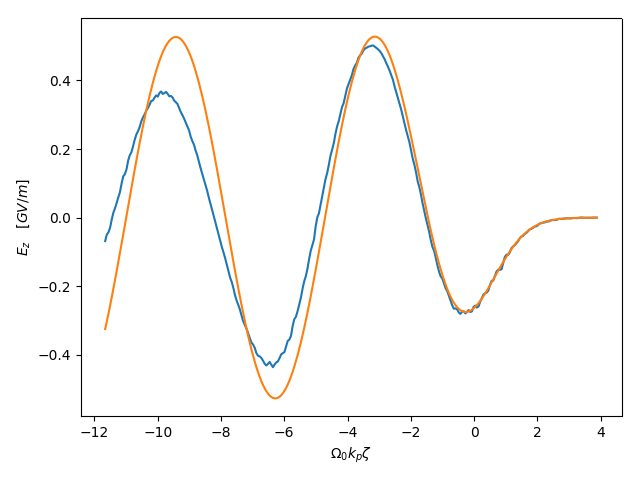
\includegraphics[width=0.7\columnwidth]{figures/analytic_vs_fbpic.png}
\caption{\protect \label{wakefields} The analytic prediction (orange) versus the FBPIC calculation (blue) for $E_z$ in the hollow channel. Horizontal axis is normalized to the eigenmode wavenumber of the $m = 0$ wake.}
\end{figure}

The hollow channel analytic theory breaks down when there is no longer a hollow channel of fixed radius. In the linear regime, where the fields are proportional to the drive bunch charge, this happens after the surface plasma wave driven by the drive bunch has time to oscillate under its own self fields, which is itself related to the channel plasma wavenumber. In this case, by $\Omega_0 k_p \zeta \approx 2 \pi$, the surface of the hollow channel has begun to evolve, and the boundary of the longitudinal electric field is falling toward the axis (see Fig.~\ref{zoomedrho}).

\begin{figure}
\centering
\subfigure{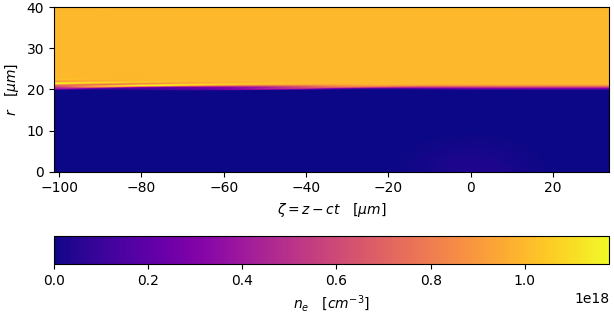
\includegraphics[width=0.7\columnwidth]{figures/rho.png}}
\subfigure{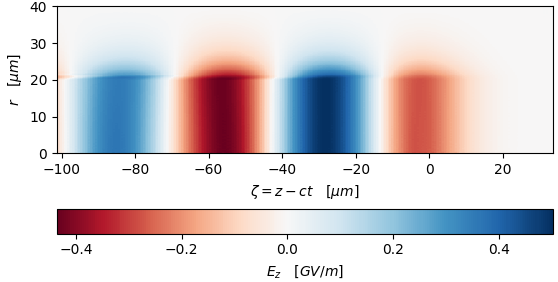
\includegraphics[width=0.7\columnwidth]{figures/Ez.png}}
\caption{\protect \label{dens_and_fields} Electron density (top) and $E_z$ (bottom)}
\end{figure}

The failure of the hollow plasma channel theory after some distance has also been observed in other simulations and experiments. Work by Lindstr{\o}m \emph{et al.}~\cite{lindstrom_etal:2018} have measured the breakdown of, in particular, the dipole wake function for distances trailing the drive bunch. Private correspondence with Lindstr{\o}m note that there is no analytic expression for this breakdown distance, although one would be useful for studying symmetric electron-positron collider designs. This is beyond the scope of the current project.

Zooming in on the edge of the hollow channel, we can see that a surface wave has formed on the channel edge, fig.~\ref{zoomedrho}. Note that the hollow channel edge has a density ramp over a few cells, and a uniform cold start, to prevent spurious fields forming at the hard boundary edge, and this leads to the cell-scale striation in the charge density. However, the results are not sensitive to these details, and the surface plasma wave feature is persistent at higher resolution.

\begin{figure}
\centering
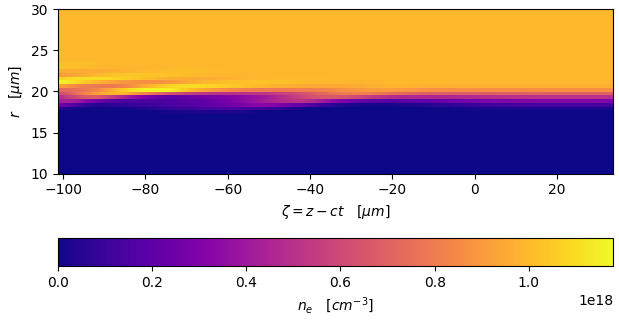
\includegraphics[width=0.7\columnwidth]{figures/zoomedrho.png}
\caption{\protect \label{zoomedrho} Electron density near the edge of the hollow plasma channel.}
\end{figure}

\section{Future Work}

We will extend this benchmark for an off-axis gaussian distribution and compare simulations with an $m=1$ mode included for (1) an on-axis gaussian distribution where we would expect $W^{(1)}$ to vanish, and (2) an off-axis gaussian distribution, where we can compute $W^{(1)}$ analytically.

\bibliography{bibliography.bib}

\end{document}